\begin{IEEEbiography}[{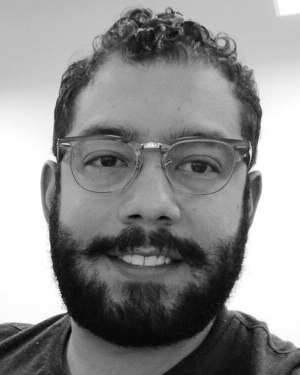
\includegraphics[width=1in,height=1.25in,clip,keepaspectratio]{../biography/yarib_300_375.jpg}}]{Yarib Nevarez} received the B.E. (Hons) degree in electronics from the Durango Institute of Technology, Durango, Mexico, in 2009, and the M.Sc. degree in Embedded Systems Design from the University of Applied Sciences Bremerhaven, Bremen, Germany, in 2017. He is currently pursuing a PhD degree with the Institute of Electrodynamics and Microelectronics, University of Bremen, Germany. His research interest is focused mainly on System-on-Chip architectures and hardware implementation for deep learning accelerators in Embedded Systems.
\\
During his professional experience, he served as a Senior Embedded Software Engineer at Texas Instruments, IBM, Continental Automotive, TOSHIBA, and Carbon Robotics. He has designed and developed software architectures for graphic calculators, automotive systems, robotic drivers, and more.
	
\end{IEEEbiography}

\begin{IEEEbiography}[{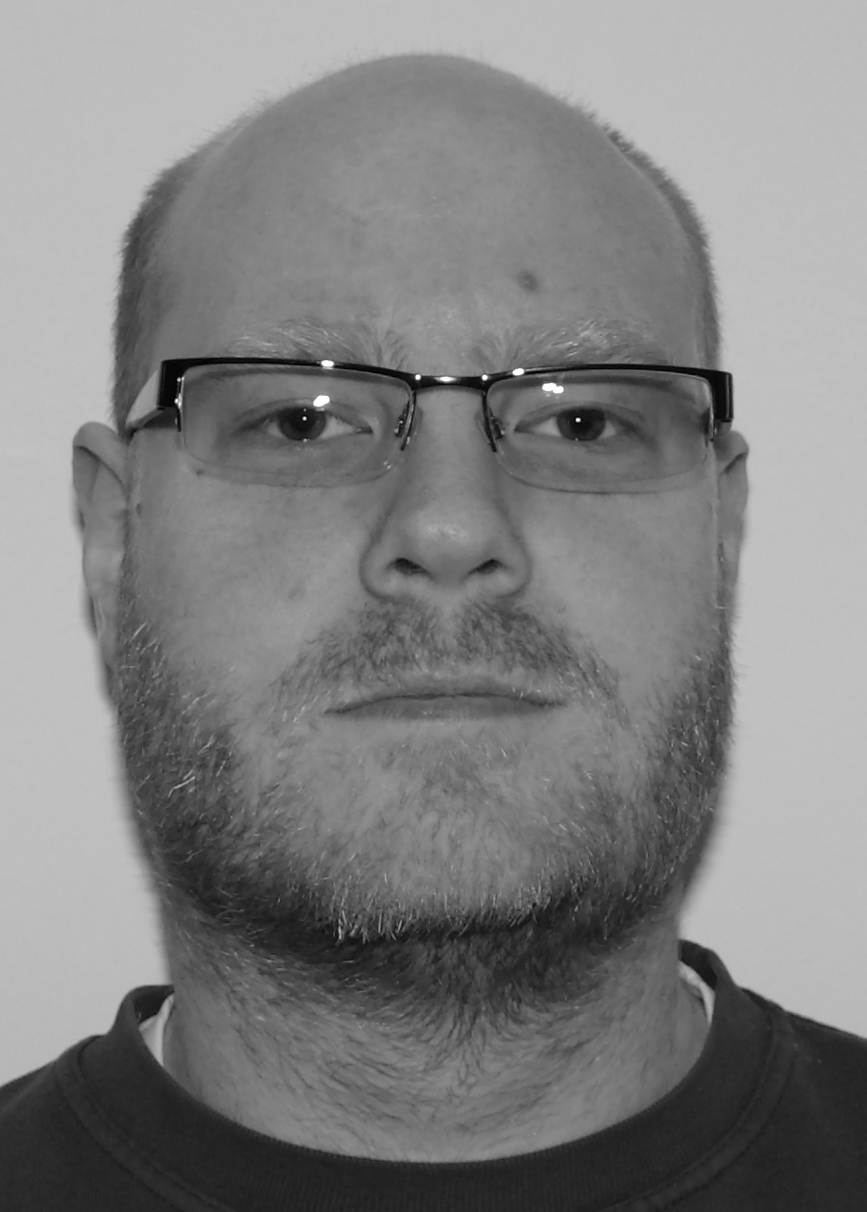
\includegraphics[width=1in,height=1.25in,clip,keepaspectratio]{../biography/Rotermund_David.jpg}}]{David Rotermund} started his scientific career as a chemical technical assistant in 1992 and received a pre-diploma in electrical engineering at the Hochschule Bremen (City University for Applied Science) in 1996. In 2002, he finished his studies of physics at the University of Bremen with a diploma (specialization in neuroscience and solid state physics). In 2007 he received his PhD "Extraction of information from the dynamical activities of neural networks". Among other neuroscience projects, he participated in several project in the field of neuro-prosthetics like the German-Israeli joint project "Models and Experiments towards Adaptive Control of Motor Prostheses" (METACOMP), the research focus Neurotechnology at the University of Bremen, and the Creative Unit "I-See: The artificial eye -- chronic wireless interface to the visual cortex". In the BMBF project KALOMED, where the goal was to design a fully wireless recording system that can be implanted under the skull of an user, he worked as project organizer and hardware/ software/ firmware designer as well as data miner. He will be the co-organizer of the upcoming Era-Net Neuron (a joint Canadian / EU project) for the development of advanced techniques in the field of visual cortex prosthesis. Beside his research in the field of neuro-prosthetics, he is keenly interested in information processing using spiking neuronal networks.
\end{IEEEbiography}

\begin{IEEEbiography}[{
\includegraphics[width=1in,height=1.25in,clip,keepaspectratio]{../biography/Klaus.jpg}}]{Klaus R. Pawelzik}
	received his PhD in the field of Nonlinear Dynamics in
	1990.  From 1991 till March 1998 he was research assistant at several
	well-known institutes in Germany and the US. Since April 1998 he is a
	tenured professor for Theoretical Physics and Theoretical Biology at the
	University of Bremen. He works mainly on topics in Theoretical
	Neuroscience, but also on problems in Neuro-technology and studies
	models of other complex adaptive systems. His many publications
	underline his expertise in these fields. Currently he is the director of
	the Center of Cognitive Sciences at the University of Bremen and has
	raised a number of third-party funds, among them several in the field of
	Neuro-technology. There he recently filed a patent with the title
	"Artificial neural network data processing apparatus and data processing
	method".
\end{IEEEbiography}

\begin{IEEEbiography}[{
\includegraphics[width=1in,height=1.25in,clip,keepaspectratio]{../biography/Alberto_Garcia-Ortiz.jpg}}]{Alberto Garcia-Ortiz}
    obtained the diploma degree in
    Telecommunication Systems from the Polytechnic University of
    Valencia (Spain) in 1998. After working for two years at Newlogic
    in Austria, he started the Ph.D. at the Institute of
    Microelectronic Systems, Darmstadt University of Technology,
    Germany. In 2003, he received from the Department of Electrical
    Engineering and Information Technology of the university the
    Ph.D. degree with "summa cum laude." From 2003 to 2005, he worked
    as a Senior Hardware Design Engineer at IBM Deutschland
    Development and Research in B{\"o}blingen.  After that he joined the
    start-up AnaFocus (Spain), where he was responsible for the design
    and integration of AnaFocus" next generation Vision
    Systems-on-Chip. He is currently full professor for the chair of
    integrated digital systems at the university of Bremen.
    Dr. Garcia-Ortiz received the "Outstanding dissertation award" in
    2004 from the European Design and Automation Association. In 2005,
    he received from IBM an innovation award for contributions to
    leakage estimation. Two patents are issued with that work. He
    serves as editor of JOLPE and is reviewer of several conferences,
    journals, and European projects. \\
    His interests include low-power
    design and estimation, communication- centric design, SoC
    integration, and variations-aware design. 
\end{IEEEbiography}
